\chapter{Evaluation}
\label{chap-five}
\newcommand{\ctheaders}[8]%
{\begin{tabular}{r|ccc||ccc|}
% Headers:
 \multicolumn{1}{r}{} & \multicolumn{3}{c}{#1}
      & \multicolumn{3}{c}{#2} \\ \cline{2-7}
% Row 1:
 #3 % \hspace{\cta}
      & \hspace{\cta} & #5 & \hspace{\cta}
      & \hspace{\cta} & #7 & \hspace{\cta}\ctstrut \\ \cline{2-7}
% Row 2:
 #4 % \hspace{\cta}
      & \hspace{\cta} & #6 & \hspace{\cta}
      & \hspace{\cta} & #8 & \hspace{\cta}\ctstrut \\ \cline{2-7}
\end{tabular}}

We have tried many approaches to summarize micro blogs. We also described a modified version of KMeans which can summarize tweets. We have evaluated the performance of our Modified KMeans algorithm against a published algorithm called SUMMALLTEXT\cite{DBLP:conf/icwsm/ChakrabartiP11}. We have built a web application which can interface with the different components needed to do the evaluation. We describe the evaluation application, the experiment and the results of the experiment in this section.

\section{Experiment Setup}
Evaluation application is a Ruby on Rails framework based application. It is connected to a Redis key value store as shown in the figure \ref{fig:evalapp1}, It acts as the data source for this application. Using a key value store like Redis provides a lot of flexibility when compared to regular relational databases. The application is designed to access tweets from three different sources, First source is directly through the Twitter API. The second data source is the Redis data store and the third data source is plain text files. Once a set of tweets are extracted from twitter they are stored in Redis too for future use. This reduces the time lag in fetching data, It also helps in serving the same set of tweets to different users for different opinions about summary. 

\begin{figure}[hbtp]
\centering
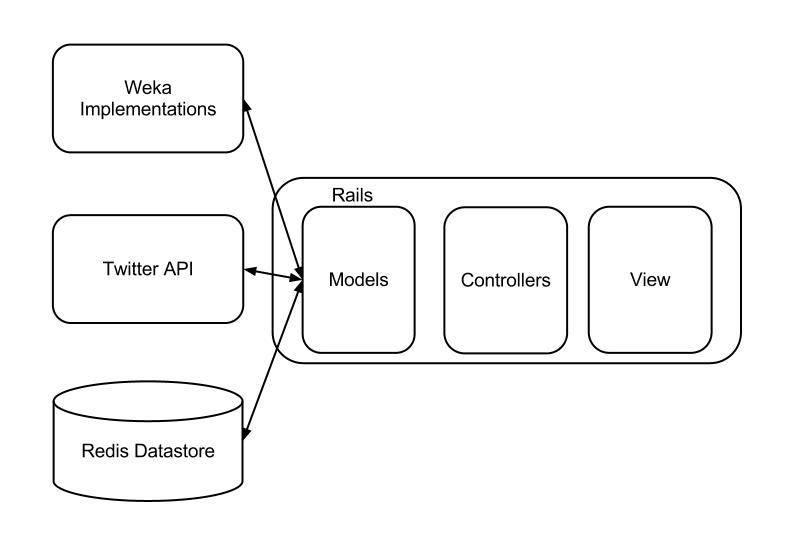
\includegraphics[width=0.9\textwidth]{Chapter-5/figs/evaluation_app_arch}
\caption{Highlevel Architecture of the Evaluation Application}
\label{fig:evalapp1}
\end{figure}

Stemming and Stopword removal was done using ruby libraries. We used a porter stemmer for stemming words. The list of stop words used for evaluation application is attached to the appendix. After stemming and stopword removal the processed tweet is formed. Then we used the ruby TF-IDF library to calculate the IDF of each word. We used the ruby bindings to the Stanford core natural language processing packages for parts of speech tagging. To compute other features we use other packages like spellchecker etc. 

The clustering algorithms are the central part of the evaluation application. We implemented two of the clustering algorithms SUMMALLTEXT and the Modified KMeans proposed by us. We wrote command line wrapper modules to Weka as shown in figure \ref{fig:evalapp1} This enables the application to make function calls to the Expectation Maximization and XMeans algorithms. The wrapper converts the features to a CSV file. Then it makes call to the appropriate algorithm using the command line and the CSV file as the input. It parses the results from a ARFF(Weka file format) file. Creates cluster objects and returns it to the Main program. The models and controllers of the Rails program make calls to the appropriate algorithms based on user preferences. The output is shown to the user on the web page. It can  also be written to a ARFF file, CSV file etc. 


\section{Experiment Description}
We treat the three phases of the experiment as being independent.
Phase 1 involves the summarization of \#BarackObama tweets, Phase 2
the summarization of \#MittRomney tweets, and Phase 3 the
summarization of a participant-chosen set of tweets from different
Twitter users.

User ratings are discrete-valued data, which means that some common
types of summary and inferential statistics used for continuous data
are inappropriate.  We adopt the conventions of HCI research in
handling Likert scale data, using the median rather than the means as
a measure of central tendency, and using non-parametric tests for
comparisons.

Bar charts of the MKM and SAT summaries for each of the three
experiments are shown below.  The median of each distribution is shown
in Table~\ref{tab:modes}.

\section{Results}

\begin{table}
\begin{center}
\begin{tabular}{|l|llllll|llllll|}
\hline
& \multicolumn{3}{c}{MKM\slash G} & \multicolumn{3}{c|}{SAT\slash G} & \multicolumn{3}{|c}{MKM\slash T} & \multicolumn{3}{c|}{SAT\slash T} \\
\hline
Phase 1: \#BarackObama      & & 4    & & & 3.75 & & & 4 & & & 3.75 & \\
Phase 2: \#MittRomney       & & 4    & & & 3    & & & 4 & & & 3  & \\
Phase 3: (participant-chosen) & & 3.5  & & & 3    & & & 3.5 & & & 3  & \\
\hline
\end{tabular}
\end{center}
\caption{Medians}
\label{tab:modes}
\end{table}

The summaries in Table~\ref{tab:modes} suggest that MKM outperforms
SAT in each of the three phases.  We can go further by analyzing
the differences between the ratings of two summaries of a specific
Twitter user, per experiment participant.  

We use a Wilcoxon signed-rank test for comparing medians: MKM versus
SAT for the General condition, and MKM versus SAT for the Topic
condition.  The non-parametric Wilcoxon test is designed for
continuous data but is applied in practice to discrete ordinal data as
well.  The hypothesis we are testing is whether there is a significant
effect of Algorithm (MKM or SAT) on the medians of the distributions
in each condition, specifically whether MKM $>$ SAT.

For Phase 1, the \#BarackObama dataset, a Wilcoxon test shows no
significant effect of Algorithm in the General condition ($W = 12.0, p
= 0.12$), and similarly no significant effect in the General condition
($W = 11.0, p = 0.18$).

For Phase 2, the \#MittRomney dataset, a Wilcoxon test shows that
there is a significant effect of Algorithm in both the General
condition ($W = 27.5, p = 0.009$) and the Topic condition ($W = 25.5,
p = 0.01$).

For Phase 3, the dataset including participant-chosen Twitter users, a
Wilcoxon test shows that there is a significant effect of Algorithm in
both the General condition ($W = 20.0, p = 0.024$) and the Topic
condition ($W = 17.0, p = 0.008$).

Alternative tests, for which the user ratings are encoded in
categorical form, show comparable results.  

For example, we can reduce the rankings into three categories, in
which MKM $<$ SAT, MKM $=$ SAT, or MKM $>$ SAT.  A $\chi^2$ test can
then be used to test the hypothesis that the probability of MKM $<$
SAT is equal to the probability of MKM $>$ SAT.  This hypothesis is
rejected in all the same cases as above.